% !TeX spellcheck = fr_FR
\chapter{Chapitre 1 : Données et format de fichier}

% \begin{center}
% 	\textit{Chaque chapitre doit commencer sur une nouvelle page.}\\*[35pt]
% \end{center}

Dans ce chapitre nous allons aborder les différents format de données qui seront
cités dans la suite de ce document.

\section{Fichier lidar}

\gls{lidar} ou en français 
détection et estimation de la distance par la lumière est une technique de mesure de distance où la lumière réalise un 
aller-retour entre sa source et un objet. On chronomètre le temps entre le moment 
où une pulsation de lumière est émise par un laser et son retour vers un capteur.
En connaissant la vitesse de propagation de la lumière dans l’environnement où elle
évolue, il est possible de déterminer la distance qui sépare l’objet 
du capteur. Plus précisément, il s’agit de la distance séparant le dispositif de
mesure et un point de l’objet frappé par la lumière émise. 
Cette opération effectuée à de multiples reprises en changeant par petit pas 
l’angle du laser, créer des points supplémentaires qui une fois réunis,
constituent un nuage de points profilant l'environnement autour de l'instrument.
Si l'instrument de mesure est placé sur un avion et que la source de lumière est
dirigée vers le bas, il est ainsi possible de capturer, sous forme d'un nuage de
points, une région du globe. Ce cas nécessite tout de fois de connaître la position
du \gls{gps} de l'avion au moment de la capture d'un point afin de mettre en relation
tous les points à la fin de la mesure.
Il existe différentes versions de la spécification et ce document va se concentrer sur la version un point deux.

Le format de stockage des nuages de points de données \gls{lidar}, est un format
binaire dont les spécifications sont définies par l'\gls{asprs}.
Le format \gls{las} est composé de trois sections, respectivement:
L'en-tête de fichier, les enregistrement à longueur variable et les données lier aux points récoltés.

\begin{table}[!h]
    \centering
    \begin{tabular}{ |c|c| }
        \hline
        En-tête \\
        \hline
        Enregistrements à longueur variable \\
        \hline
        Données des points \\
        \hline
    \end{tabular}
    \caption[Sections composant un fichier au format LAS]{
            Sections composant un fichier au format LAS, 
            Source: adapté de LAS Specification Version 1.2 (2008, p. 2)
    }
    \label{tab:las_sections}
\end{table}
\newpage
Dans toutes les sections, on défini les types de données dans le tableau \ref{tab:data_type}
\begin{table}[!htb]
    \centering
    \begin{tabular}{|l|c|}
    \hline
    \textbf{Type de donnée}           & \textbf{Nombre d'octets} \\ \hline
    char           & 1               \\ \hline
    unsigned  char & 1               \\ \hline
    short          & 2               \\ \hline
    unsigned short & 2               \\ \hline
    long           & 4               \\ \hline
    unsigned long  & 4               \\ \hline
    double \tablefootnote{selon le standard IEEE 754} & 8     \\ \hline
    \end{tabular}
    \caption[Type de données de la définition du format LAS]{
        Type de données de la définition du format LAS,
        Source: adapté de LAS Specification Version 1.2 (2008, p. 2-3)
    }
    \label{tab:data_type}
\end{table}

\subsection{En-tête publique}

L'en-tête publique comporte les métadonnées du fichier.
Il est composé de tous les champs du tableau~\ref {tab:las_header} présent dans l'annexe~1.
Tous les champs inutilisés doivent être remplis par des bits nuls et les champs sont tous en little endian.
La signature de fichier doit obligatoirement contenir les quatre caractères “LASF” et est requise par la spécification.
Un programme lisant le fichier doit vérifier cette signature pour déterminer qu’il s’agisse bien d’un fichier \gls{las}.

Parmi les champs, les facteurs $ X, Y $ et $ Z $ scale sont utilisés avec les valeurs $ X, Y$ et $Z$ offset pour obtenir des coordonnées cartésiennes des axes.
Ces valeurs sont globales au fichier. Voici la formule pour chaque coordonnée:

\begin{equation*}
    X_{coordinate} = (X_{record} * X_{scale}) + X_{offset}
\end{equation*}
\begin{equation*}
    Y_{coordinate}= (Y_{record} * Y_{scale}) + Y_{offset}
\end{equation*}
\begin{equation*}
    Z_{coordinate}= (Z_{record} * Z_{scale}) + Z_{offset}
\end{equation*}

Les champs min et max $X, Y, Z$ sont les valeurs minimales et maximales non mise à l'échelle des données des points présent dans la dernière section du fichier.

\subsection{Enregistrements à longueur variable}

Ce bloc suit directement l'en-tête de fichier et peut avoir une ou plusieurs entrées.
Le nombre total d'entrée est spécifié dans le champs "Number of Variable Length Records" de l'en-tête de fichier.
Ce bloc doit être lu de manière séquentielle car chaque entrée est de taille variable.
Chaque entrée est débutée par une en-tête de 54 octets selon le tableau \ref{tab:las_var_record_header}

\begin{table}[!htb]
\centering
\begin{tabular}{|l|l|c|c|}
\hline
\multicolumn{1}{|c|}{\textbf{Champ}} & \multicolumn{1}{c|}{\textbf{Type de donnée}} & \textbf{Taille (Octets)} & \textbf{Requis} \\ \hline
Réservé                              & unsigned short                               & 2                        &                 \\ \hline
User ID                              & char{[}16{]}                                 & 16                       & *               \\ \hline
Record ID                            & unsigned short                               & 2                        & *               \\ \hline
Record Lenght After Header           & unsigned short                               & 2                        & *               \\ \hline
Description                          & char{[}32{]}                                 & 32                       &                 \\ \hline
\end{tabular}
\caption{
Champs de l'en-tête des enregistrement de longueur variable.
Source: adapté de LAS Specification Version 1.2 (2008, p. 6)}
\label{tab:las_var_record_header}
\end{table}

Les enregistrements peuvent provenir de sources différentes.
Elles sont identifiées dans le par le champ "User ID" qui est une chaîne de caractères unique et enregistrée auprès d'une organisation afin de prévenir que deux sources différentes aie la même séquence.

Chaque utilisateur dispose de 65536 enregistrements au maximum qu'il gère de manière indépendante.
Les identifiants des enregistrement sont renseigné dans le champ "Record ID" de l'en-tête.
Il peut également, s'il le souhaite, publier un signification lié aux identifiants d'enregistrement.

"Record Lenght After Header": il s'agit d'un offset en nombre d'octets qui indique l'endroit où commence les données aprés l'en-tête de 54 bytes.
La source des données peut renseigner des informations supplémentaires dans l'en-tête mais elles ne suivront pas le standard de la spécification.

\subsection{Données des points}
Les données des points commencent à l'adresse du champ "Offset to Point Data" de l'en-tête de fichier.
Il existe quatre formats pour les entrées de point. 

Le format zero est le plus commun. 

\section{Fichier Stéréoligraphique}

Le format de fichier \gls{stl} est conçu par la société 3D System pour contenir des modèles d'objets tridimensionnelles.
Il a été pensé pour permettre un prototypage rapide dans les logiciels de \gls{cao}. 
Ce format ne décrit que la géométrie de la surface d'un modèle.
Il existe un format binaire et un format ascii, le dernier laissant une empreinte dans la mémoire morte plus conséquente.

On y stock les triangles composant le modèle où chaque sommet du triangle est décrit par ses coordonnées cartésienne $(x,y,z)$. Chaque triangle partage, sans exception, deux sommets avec un triangle voisin.
La coordonnée dans l'axe $z$ est considérée comme l'axe vertical, ceci peut être gênant pour les programmes considérant l'axe $y$ comme l'axe vertical.

\subsection{Format ASCII}

Le format commence par la séquence de caractères : "solid \textit{nom}" où \textit{nom} est une séquence correspondant au nom du modèle qui est facultatif.
Si le nom est vide, l'espace après "solid" est obligatoire.
Un triangle s'écrit de la manière suivante :
\begin{lstlisting}[frame=single, escapechar=\%]
facet normal % $n_x$% %$n_y$% %$n_z$%
    outer loop
        vertex %$v1_x$% %$v1_y$% %$v1_z$%
        vertex %$v2_x$% %$v2_y$% %$v2_z$%
        vertex %$v3_x$% %$v3_y$% %$v3_z$%
    endloop
endfacet
\end{lstlisting}
Les sommets sont définis à l'aide du mot clé "vertex" qui sont contenus dans un block loop. Les $n$ et les $v$ sont des nombres à virgule flotante.
Ils s'écrivent dans le format "signe-mantisse-e-signe-exposant", par exemple "6.248000e-003".
La fin du fichier ascii est définie par la séquence : "end solid".

\subsection{Format binaire}

\section{Fichier VTK}

% \begin{figure}[tbph!]
% 	\centering
% 	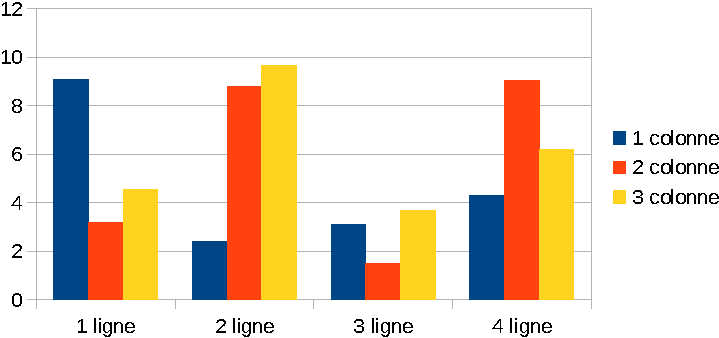
\includegraphics[width=0.7\linewidth]{chart}
% 	\caption[Diagramme machin]{Diagramme machin. Source : tiré de Tartempion 2010, p. 42 / tiré de ce-site.ch, ref. URL01 / réalisé par Nom Prénom.}
% 	\label{fig:chart1}
% \end{figure}
% 
% 
% \begin{table}[tbph!]
% 	\centering{
% 		\begin{tabular}{ |l|c|c|c| }
% 			\hline
% 			& \textbf{Condition 1} & \textbf{Condition 2} & \textbf{Condition 3} \\
% 			\hline
% 			\textbf{Test 1} & X & O & X \\
% 			\hline
% 			\textbf{Test 2} & O & X & X \\
% 			\hline
% 			\textbf{Test 3} & O & X & O \\
% 			\hline 
% 		\end{tabular}
% 		\caption[Lot de données n°1]{Lot de données n°1. Source: tiré de Tartempion 2010, p. 42 / tiré de ce-site.ch, ref. URL02 / réalisé par Nom Prénom.}
% 		\label{tab:tableau1}
% 	}
% \end{table}
% 
% 
% \begin{figure}[tbph!]
% 	\centering
% 	
\includegraphics[width=0.7\linewidth]{diagram}
% 	\caption[Schéma bidule.]{Schéma bidule. Source : tiré de Tartempion 2010, p. 42 / tiré de ce-site.ch, ref. URL03 / réalisé par Nom Prénom.}
% 	\label{fig:diagram}
% \end{figure}
% 
% 
% \section{Titre de niveau 2}
% 
% 
% \begin{figure}[tbph!]
% 	\centering
% 	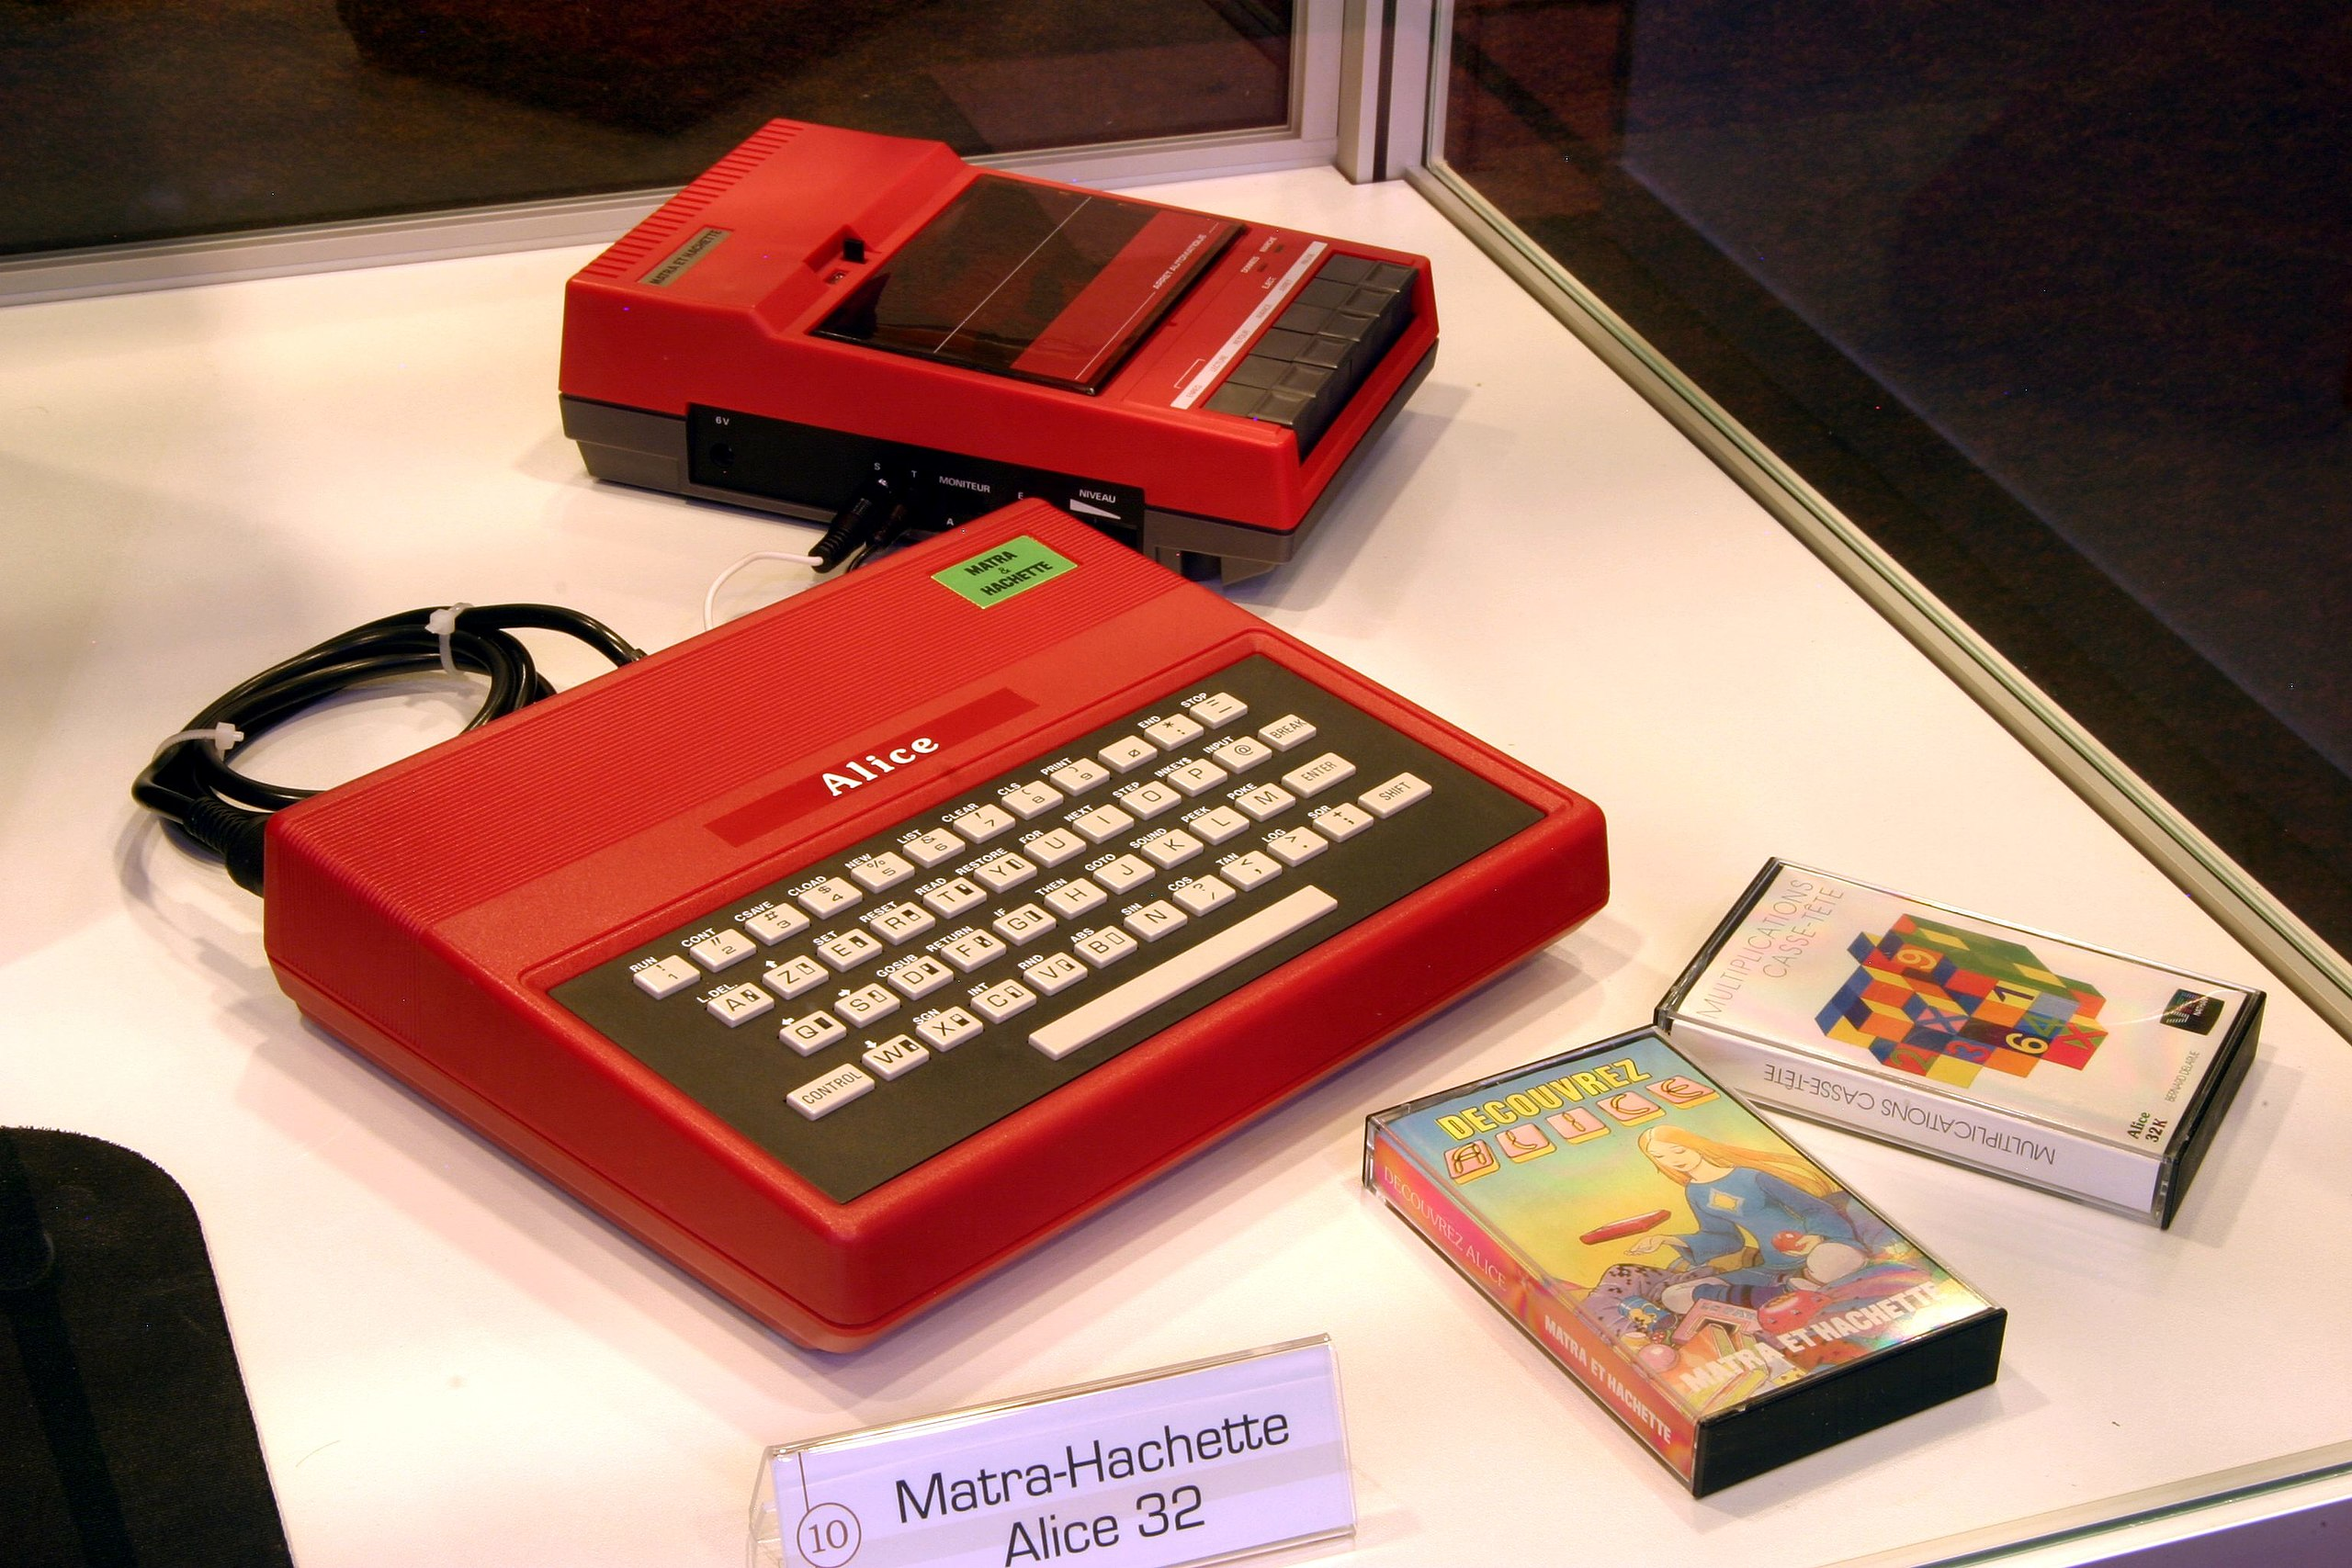
\includegraphics[width=0.7\linewidth]{ordi}
% 	\caption[Alice, Micro-ordinateur MATRA.]{Alice, Micro-ordinateur MATRA. Source : tiré de Tartempion 2010, p. 42 / tiré de ce-site.ch, ref. URL03 / réalisé par Nom Prénom.}
% 	\label{fig:image}
% \end{figure}
% 
% 
% \subsection{Titre de niveau 3}
% 
% 
% \begin{table}[tbph!]
% 	\centering{
% 		\begin{tabular}{ |l|c|c|c| }
% 			\hline
% 			& \textbf{Condition 1} & \textbf{Condition 2} & \textbf{Condition 3} \\
% 			\hline
% 			\textbf{Test 1} & X & O & X \\
% 			\hline
% 			\textbf{Test 2} & O & X & X \\
% 			\hline
% 			\textbf{Test 3} & O & X & O \\
% 			\hline 
% 		\end{tabular}
% 		\caption[Lot de données n°2.]{Lot de données n°2. Source: tiré de Tartempion 2010, p. 42 / tiré de ce-site.ch, ref. URL05 / réalisé par Nom Prénom.}
% 		\label{tab:tableau2}
% 	}
% \end{table}
